\documentclass{standalone}
\usepackage{tikz}
\usetikzlibrary{patterns}
\usetikzlibrary{positioning}
\usetikzlibrary{patterns, positioning}
\usetikzlibrary{shapes.misc}
\usepackage[outline]{contour}
\contourlength{1.5pt} 
\usepackage[sfdefault]{ClearSans}

\begin{document}
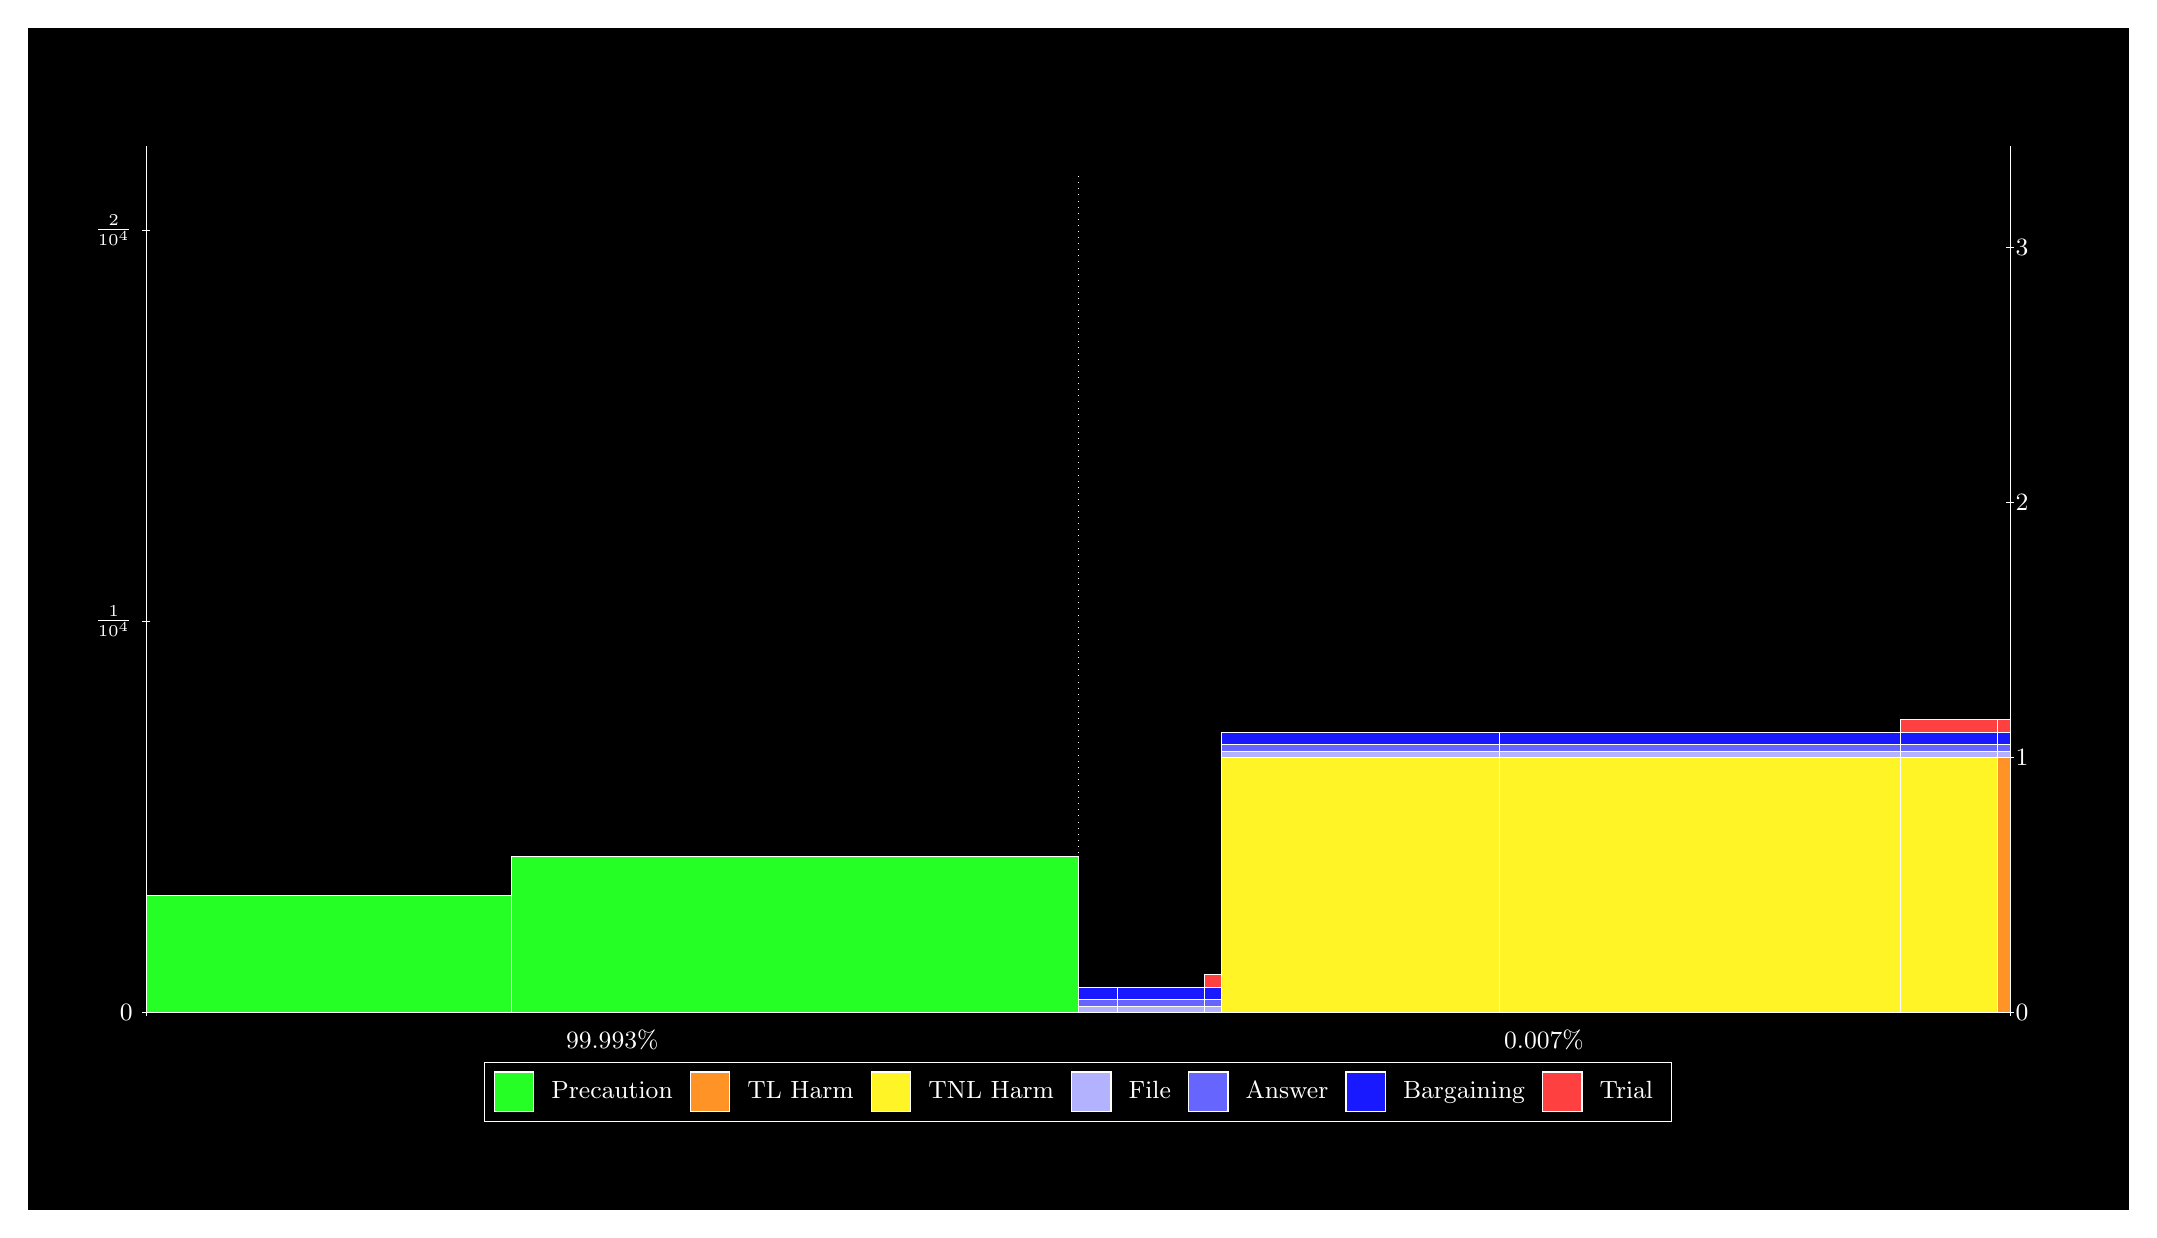
\begin{tikzpicture}
\draw[fill=black] (0,0) rectangle (26.667,15);
\draw[fill=green!85,draw=white,very thin] (1.5,2.5) rectangle (6.1372,3.9906);
\draw[fill=green!85,draw=white,very thin] (6.1372,2.5) rectangle (13.333,4.4874);
\draw[fill=green!85,draw=white,very thin] (13.333,2.5) rectangle (13.828,2.5001);
\draw[fill=blue!30,draw=white,very thin] (13.333,2.5001) rectangle (13.828,2.5811);
\draw[fill=blue!60,draw=white,very thin] (13.333,2.5811) rectangle (13.828,2.6621);
\draw[fill=blue!90,draw=white,very thin] (13.333,2.6621) rectangle (13.828,2.824);
\draw[fill=green!85,draw=white,very thin] (13.828,2.5) rectangle (14.932,2.5001);
\draw[fill=blue!30,draw=white,very thin] (13.828,2.5001) rectangle (14.932,2.5811);
\draw[fill=blue!60,draw=white,very thin] (13.828,2.5811) rectangle (14.932,2.6621);
\draw[fill=blue!90,draw=white,very thin] (13.828,2.6621) rectangle (14.932,2.8241);
\draw[fill=green!85,draw=white,very thin] (14.932,2.5) rectangle (15.148,2.5001);
\draw[fill=blue!30,draw=white,very thin] (14.932,2.5001) rectangle (15.148,2.5811);
\draw[fill=blue!60,draw=white,very thin] (14.932,2.5811) rectangle (15.148,2.6621);
\draw[fill=blue!90,draw=white,very thin] (14.932,2.6621) rectangle (15.148,2.824);
\draw[fill=red!75,draw=white,very thin] (14.932,2.824) rectangle (15.148,2.986);
\draw[fill=green!85,draw=white,very thin] (15.148,2.5) rectangle (18.679,2.5001);
\draw[fill=yellow!85,draw=white,very thin] (15.148,2.5001) rectangle (18.679,5.7395);
\draw[fill=blue!30,draw=white,very thin] (15.148,5.7395) rectangle (18.679,5.8204);
\draw[fill=blue!60,draw=white,very thin] (15.148,5.8204) rectangle (18.679,5.9014);
\draw[fill=blue!90,draw=white,very thin] (15.148,5.9014) rectangle (18.679,6.0634);
\draw[fill=green!85,draw=white,very thin] (18.679,2.5) rectangle (18.688,2.5001);
\draw[fill=orange!85,draw=white,very thin] (18.679,2.5001) rectangle (18.688,5.7395);
\draw[fill=blue!30,draw=white,very thin] (18.679,5.7395) rectangle (18.688,5.8204);
\draw[fill=blue!60,draw=white,very thin] (18.679,5.8204) rectangle (18.688,5.9014);
\draw[fill=blue!90,draw=white,very thin] (18.679,5.9014) rectangle (18.688,6.0634);
\draw[fill=green!85,draw=white,very thin] (18.688,2.5) rectangle (23.781,2.5001);
\draw[fill=yellow!85,draw=white,very thin] (18.688,2.5001) rectangle (23.781,5.7395);
\draw[fill=blue!30,draw=white,very thin] (18.688,5.7395) rectangle (23.781,5.8205);
\draw[fill=blue!60,draw=white,very thin] (18.688,5.8205) rectangle (23.781,5.9015);
\draw[fill=blue!90,draw=white,very thin] (18.688,5.9015) rectangle (23.781,6.0634);
\draw[fill=green!85,draw=white,very thin] (23.781,2.5) rectangle (25.012,2.5001);
\draw[fill=yellow!85,draw=white,very thin] (23.781,2.5001) rectangle (25.012,5.7395);
\draw[fill=blue!30,draw=white,very thin] (23.781,5.7395) rectangle (25.012,5.8204);
\draw[fill=blue!60,draw=white,very thin] (23.781,5.8204) rectangle (25.012,5.9014);
\draw[fill=blue!90,draw=white,very thin] (23.781,5.9014) rectangle (25.012,6.0634);
\draw[fill=red!75,draw=white,very thin] (23.781,6.0634) rectangle (25.012,6.2254);
\draw[fill=green!85,draw=white,very thin] (25.012,2.5) rectangle (25.167,2.5001);
\draw[fill=orange!85,draw=white,very thin] (25.012,2.5001) rectangle (25.167,5.7395);
\draw[fill=blue!30,draw=white,very thin] (25.012,5.7395) rectangle (25.167,5.8204);
\draw[fill=blue!60,draw=white,very thin] (25.012,5.8204) rectangle (25.167,5.9014);
\draw[fill=blue!90,draw=white,very thin] (25.012,5.9014) rectangle (25.167,6.0634);
\draw[fill=red!75,draw=white,very thin] (25.012,6.0634) rectangle (25.167,6.2254);
\draw[white,very thin] (1.5,2.5) -- (1.5,13.5);
\draw[white,very thin] (1.45,2.5) -- (1.55,2.5);
\node[font=\small,text=white, anchor=east] at (1.45, 2.5) {0};
\draw[white,very thin] (1.45,7.4686) -- (1.55,7.4686);
\node[font=\small,text=white, anchor=east] at (1.45, 7.4686) {$\frac{1}{10^{4}}$};
\draw[white,very thin] (1.45,12.437) -- (1.55,12.437);
\node[font=\small,text=white, anchor=east] at (1.45, 12.437) {$\frac{2}{10^{4}}$};

\draw[white,dotted,very thin] (13.333,2.83) -- (13.333,13.17);
\draw[white,very thin] (25.167,2.5) -- (25.167,13.5);
\draw[white,very thin] (25.117,2.5) -- (25.217,2.5);
\node[font=\small,text=white, anchor=west] at (25.117, 2.5) {0};
\draw[white,very thin] (25.117,5.7394) -- (25.217,5.7394);
\node[font=\small,text=white, anchor=west] at (25.117, 5.7394) {1};
\draw[white,very thin] (25.117,8.9787) -- (25.217,8.9787);
\node[font=\small,text=white, anchor=west] at (25.117, 8.9787) {2};
\draw[white,very thin] (25.117,12.218) -- (25.217,12.218);
\node[font=\small,text=white, anchor=west] at (25.117, 12.218) {3};

\draw[white,very thin] (1.5,2.5) -- (25.167,2.5);
\draw[white,very thin] (1.5,2.45) -- (1.5,2.55);
\node[font=\small,text=white, anchor=north] at (1.5, 2.45) {};
\draw[white,very thin] (25.167,2.45) -- (25.167,2.55);
\node[font=\small,text=white, anchor=north] at (25.167, 2.45) {};

\node[font=\small,text=white,anchor=south] at (7.4167, 1.9) {99.993\%};
\node[font=\small,text=white,anchor=south] at (19.25, 1.9) {0.007\%};
\draw (13.3333,2.5) node (B) {};
\begin{scope}[align=center]
\matrix[scale=0.5,draw=white,below=0.5cm of B,nodes={draw},column sep=0.1cm]{
\node[rectangle,draw,minimum width=0.5cm,minimum height=0.5cm,fill=green!85]{}; & \node[draw=none,font=\small,text=white]{Precaution}; &
\node[rectangle,draw,minimum width=0.5cm,minimum height=0.5cm,fill=orange!85]{}; & \node[draw=none,font=\small,text=white]{TL Harm}; &
\node[rectangle,draw,minimum width=0.5cm,minimum height=0.5cm,fill=yellow!85]{}; & \node[draw=none,font=\small,text=white]{TNL Harm}; &
\node[rectangle,draw,minimum width=0.5cm,minimum height=0.5cm,fill=blue!30]{}; & \node[draw=none,font=\small,text=white]{File}; &
\node[rectangle,draw,minimum width=0.5cm,minimum height=0.5cm,fill=blue!60]{}; & \node[draw=none,font=\small,text=white]{Answer}; &
\node[rectangle,draw,minimum width=0.5cm,minimum height=0.5cm,fill=blue!90]{}; & \node[draw=none,font=\small,text=white]{Bargaining}; &
\node[rectangle,draw,minimum width=0.5cm,minimum height=0.5cm,fill=red!75]{}; & \node[draw=none,font=\small,text=white]{Trial}; \\\\
};\end{scope}

\end{tikzpicture}
\end{document}